\documentclass[a0paper,portrait]{baposter}



\usepackage{wrapfig}
\usepackage{lmodern}

\usepackage[utf8]{inputenc} %unicode support
\usepackage[T1]{fontenc}

% \usepackage[showframe=true]{geometry}
\usepackage{enumitem}  % for zero indentation of itemizes 
\usepackage{xcolor}  % for equation 

\selectcolormodel{cmyk}

\graphicspath{{figures/}} % Directory in which figures are stored


\newcommand{\compresslist}{%
\setlength{\itemsep}{0pt}%
\setlength{\parskip}{1pt}%
\setlength{\parsep}{0pt}%
}

\newenvironment{boenumerate}
  {\begin{enumerate}\renewcommand\labelenumi{\textbf\theenumi.}}
  {\end{enumerate}}



\begin{document}


\definecolor{darkgreen}{cmyk}{0.8,0,0.8,0.45}
\definecolor{lightgreen}{cmyk}{0.8,0,0.8,0.25}

\begin{poster}
{
grid=false,
headerborder=open, % Adds a border around the header of content boxes
colspacing=1em, % Column spacing
bgColorOne=white, % Background color for the gradient on the left side of the poster
bgColorTwo=white, % Background color for the gradient on the right side of the poster
borderColor=darkgreen, % Border color
headerColorOne=lightgreen, % Background color for the header in the content boxes (left side)
headerColorTwo=lightgreen, % Background color for the header in the content boxes (right side)
headerFontColor=white, % Text color for the header text in the content boxes
boxColorOne=white, % Background color of the content boxes
textborder=rounded, %rectangle, % Format of the border around content boxes, can be: none, bars, coils, triangles, rectangle, rounded, roundedsmall, roundedright or faded
eyecatcher=false, % Set to false for ignoring the left logo in the title and move the title left
headerheight=0.11\textheight, % Height of the header
headershape=rounded, % Specify the rounded corner in the content box headers, can be: rectangle, small-rounded, roundedright, roundedleft or rounded
headershade=plain,
headerfont=\Large\textsf, % Large, bold and sans serif font in the headers of content boxes
%textfont={\setlength{\parindent}{1.5em}}, % Uncomment for paragraph indentation
linewidth=2pt % Width of the border lines around content boxes
}
{}
%
%----------------------------------------------------------------------------------------
%	TITLE AND AUTHOR NAME
%----------------------------------------------------------------------------------------
%
{
\textsf %Sans Serif
{Dynamic Beam Search in\\Sequence-to-Sequence Models
}
} % Poster title
% {\vspace{1em} Marta Stepniewska, Pawel Siedlecki\\ % Author names
% {\small \vspace{0.7em} Department of Bioinformatics, Institute of Biochemistry and Biophysics, PAS, Warsaw, Pawinskiego 5a}} % Author email addresses
{\sf\vspace{0.5em}\\
Yu-Hsiang Lin, Shuxin Lin, Hai Pham
\vspace{0.1em}\\
\small{Language Technologies Institute, Carnegie Mellon University
\vspace{0.2em}\\
$\{$yuhsianl, shuxinl, htpham$\}$@andrew.cmu.edu}
}
	{
\includegraphics[width=6.5cm]{LTI-logo.png}} % University/lab logo


\headerbox{1.~Introduction}{name=introduction,column=0,row=0, span=3}{
Sequence-to-sequence (seq2seq) models are typically trained by the maximum likelihood estimation with the ``teacher forcing'' technique, and beam search is used to accelerate the test-time decoding. While beam search has an advantage over greedy search for accuracy, it is time consuming as the beam size increases. We aim to address this problem and propose two methods of adapting the beam size for decoding: (1) \textbf{deterministic (heuristic) agent} with a fixed threshold and (2) \textbf{dynamic asynchronous actor-critic agent}. 
}


\headerbox{2.~Seq2Seq with Fixed Attention}{name=model,column=0,below=introduction,span=1}{

\begin{itemize}[leftmargin=*]
\item Seq2seq model are both LSTM RNNs, except that the encoder is \textit{bi-directional}
\item Input augmentation with GLoVe word embedding 
\item We use the ``fixed'' attention, by which we attend at $h^{enc}_t$ when decoding for $h^{dec}_t$. 
  \[
      p_{y_{\textcolor{red}{t}}} = softmax(W_{s} \cdot attn(h^{dec}_{\textcolor{red}{t}}, h^{enc}) + b_{s}) \label{eq:pt_attn}
  \]
where attention is: 
  \[
      attn(h^{dec}_{\textcolor{red}{t}}, h^{enc}) = h^{enc}_{\textcolor{red}{t}}
  \]

\end{itemize}

  
\begin{center}
    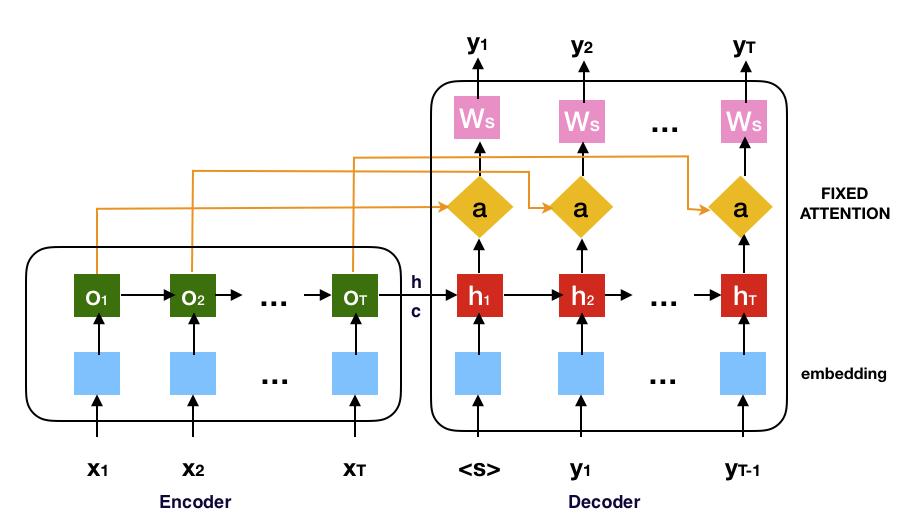
\includegraphics[width=\linewidth]{fixed_attention.png}
	\small{Fixed attention architecture}
\end{center}

}


\headerbox{3.~Search with Fixed Beam Size}{name=beam,column=0,below=model,span=1}{
% In the test time, decoding the most likely output sequence involves searching through all the possible output sequences based on their likelihood. One popular heuristic is the beam search, which is an extension to the greedy search and returns a list of most likely output sequences by measuring accumulated log probability at each step. Larger beam size potentially results in better performance of a model as the multiple candidate sequences increase the likelihood of better matching a target sequence. However, this increased performance results in a decrease in decoding speed.

\begin{itemize}[leftmargin=*]
	\item Beam search is the traditional way to handle search in decode time 
    \item Trade processing time with the accuracy compared to greedy search; it always process $|B| * |V_{label}|$ tokens at each time step
    \item Time and resource hungry if the label size is big 
\end{itemize}

%\begin{center}
%    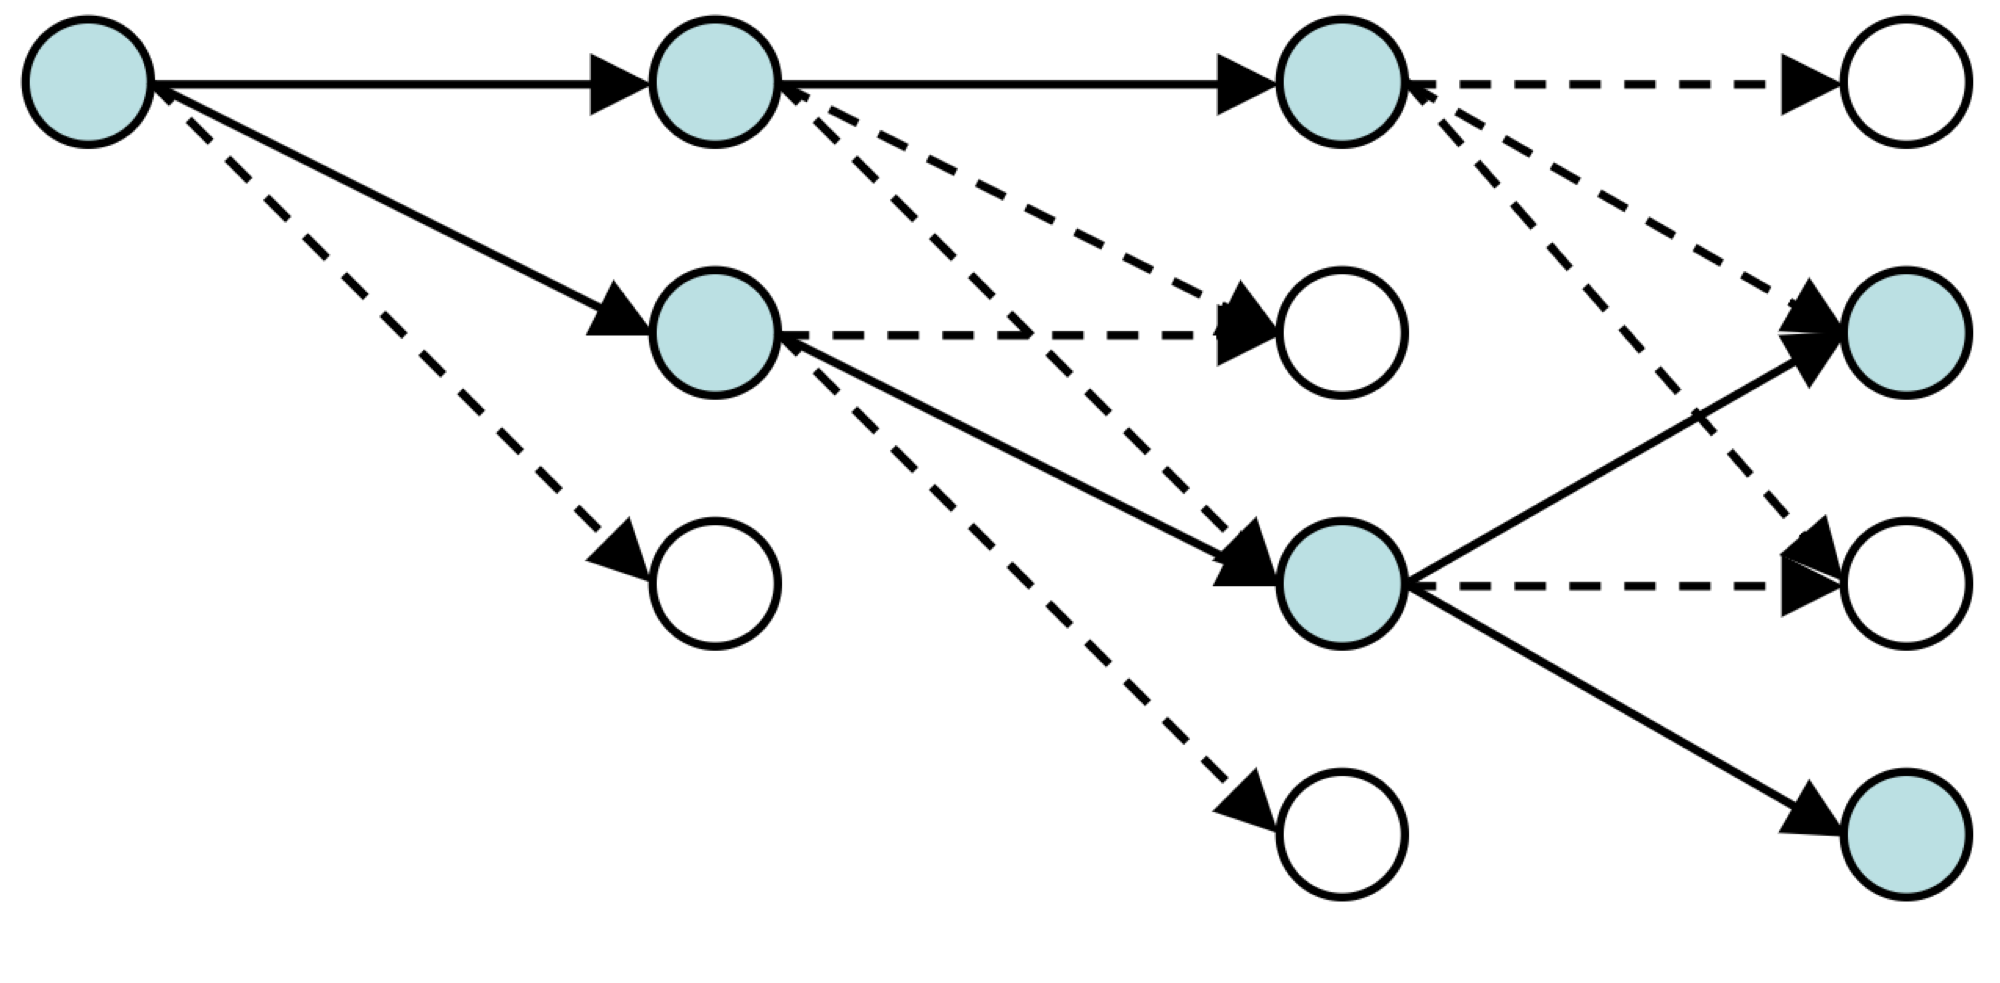
\includegraphics[width=\linewidth]{hard_beam_2.png}
%    \small{Hard Beam Search with Size=2}
%\end{center}

}

\headerbox{4.~Heuristic Pruning and Growing for Dynamic Beam Search}{name=heuristic,span=2,column=1,below=introduction}{ % To reduce this block to 1 column width, remove 'span=2'

\begin{itemize}[leftmargin=*]
\item Current beam size $B$ at step $t$
\item $B \rightarrow B-1$ $\;$ if $\;$ $\sum_t \log P(y^{B}_t) - \sum_t \log P(y^{0}_t) \leq \log r^{sen}_{low}$ $\;$ or $\;$ $\log P(y^{B}_t) - \log P(y^{0}_t) \leq \log r^{word}_{low}$
\item $B \rightarrow B+1$ $\;$ if $\;$ $\sum_t \log P(y^{B+1}_t) - \sum_t \log P(y^{0}_t) > \log r^{sen}_{low}$ $\;$ or $\;$ $\log P(y^{B+1}_t) - \log P(y^{0}_t) > \log r^{word}_{low}$
\end{itemize}

}


\headerbox{5.~Reinforcement Learning for Dynamic Beam Search}{name=env,span=2,column=1,below=heuristic}{ % To reduce this block to 1 column width, remove 'span=2'

\begin{itemize}[leftmargin=*]
\item Design the states, actions, and rewards for dynamic beam decoding
\end{itemize}

\begin{center}
    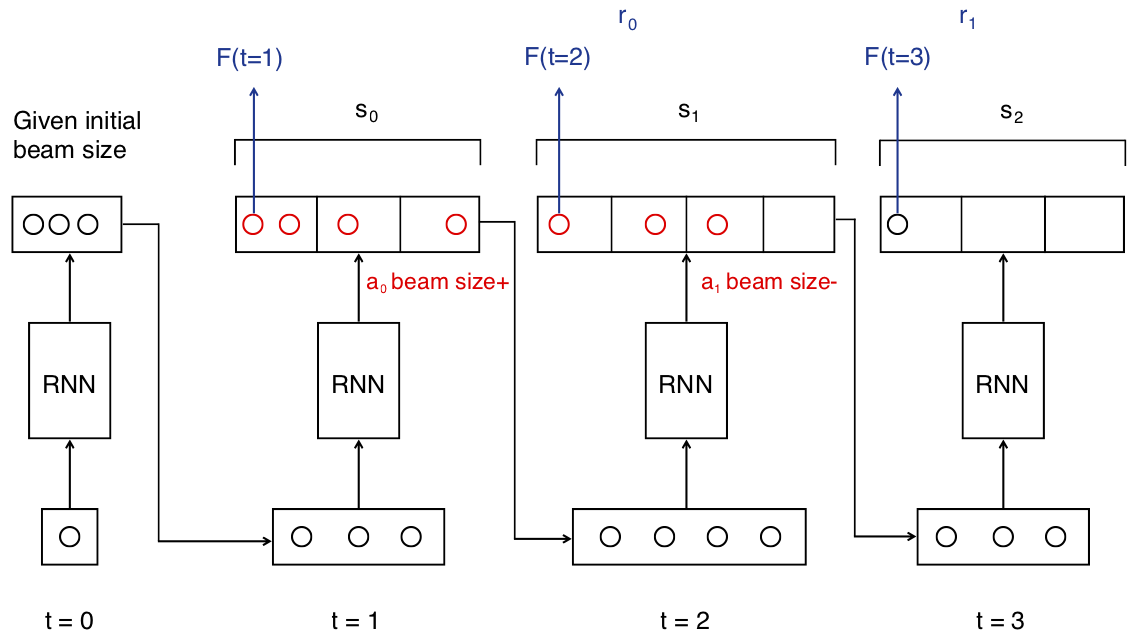
\includegraphics[width=0.7\linewidth]{adapt2.png}
\end{center}

}



\headerbox{6.~Training Decoder with Asynchronous Actor-Critic}{name=a3c,span=2,column=1,below=env}{ % To reduce this block to 1 column width, remove 'span=2'

% After the encoder-decoder model is trained using supervised learning, we further learn the policy that dynamically adjusts the beam size using reinforcement learning. We use the actor-critic model and policy gradient to train the policy network. The actor network is pre-trained by imitation learning using the experience generated by the heuristic pruning and growing rules.

% In the seq2seq environment, an episode consists of a sequence. Our state consists of the top-$k$ log probabilities and accumulated log probabilities, as well as the current beam size. The action space of the agent is 3:~increasing or decreasing the beam size by 1 (limited by maximum and minimum beam sizes), or remain the same beam size. The learning goal of the policy is to decrease the beam size as much as possible, while increase the decoding F-score as much as possible. The reward is therefore a combination of two factors:~if the beam size is decreased (increased) or the partial F-score is increased (decreased) at this $(s_t, a_t, s_{t+1})$ transition, the agent obtains a positive (negative) reward.
\begin{center}
    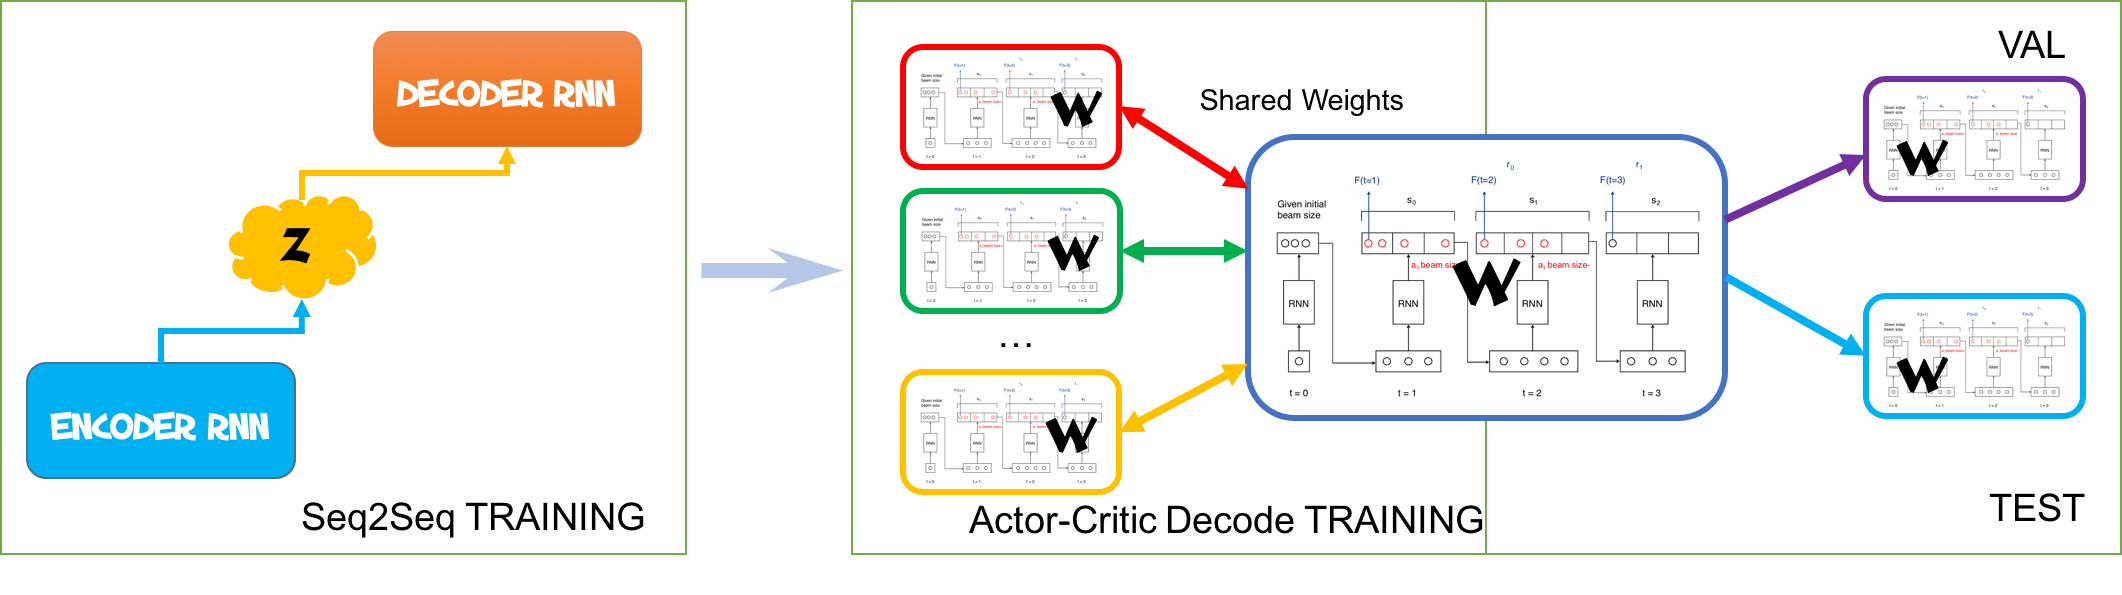
\includegraphics[width=\linewidth]{figures/actor_critic.png}
	\small{Asynchronous Actor-Critic (A3C) REINFORCE \cite{mnih2016asynchronous} with many shared-weights training agents}
\end{center}





%\hspace{0pt}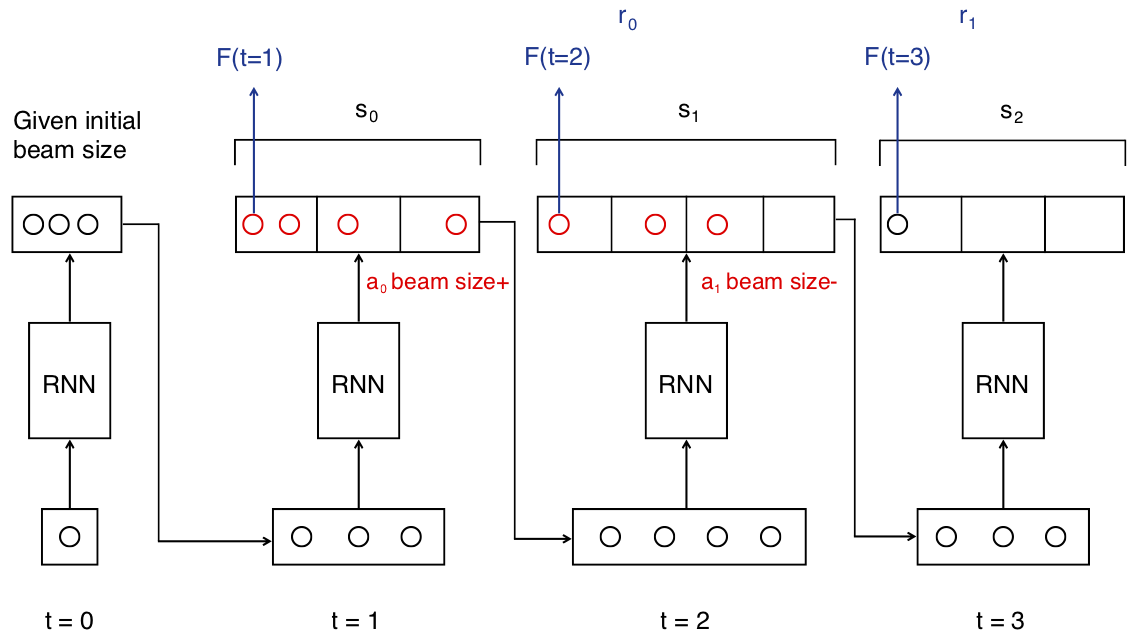
\includegraphics[width=0.95\linewidth]{adapt2.png}

%\begin{wrapfigure}{l}{0.3\textwidth}
%    \vspace{10pt}
%    \begin{center}
%        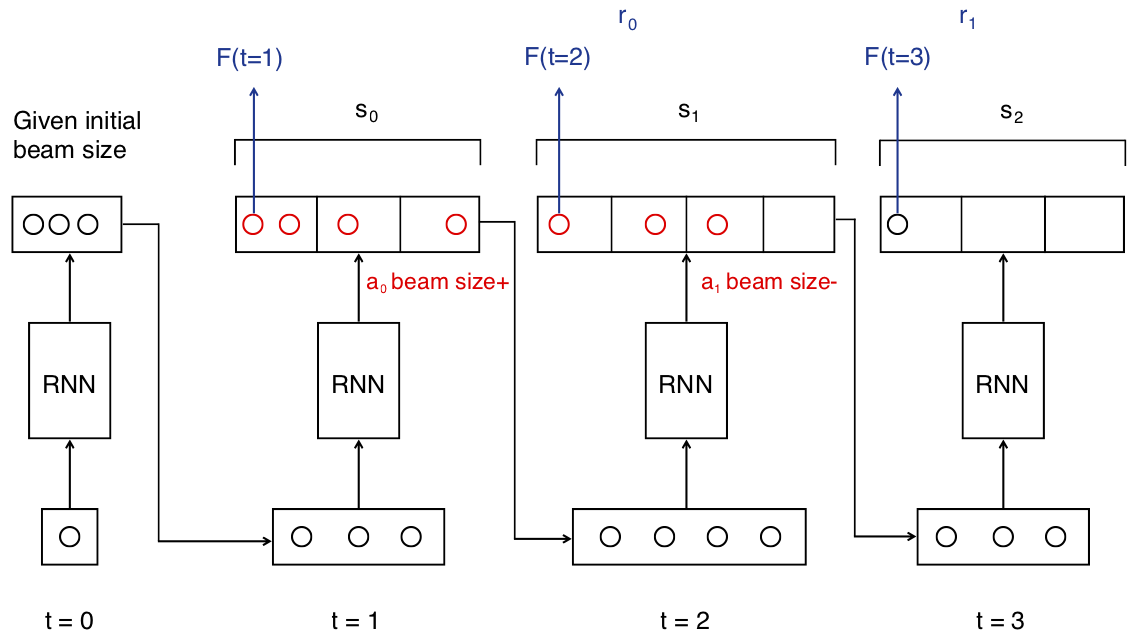
\includegraphics[width=\linewidth]{adapt2.png}
%    \end{center}
%    %\vspace{-145pt}
%\end{wrapfigure}

}



\headerbox{7.~Experiment Results}{name=result,column=1,below=a3c,span=2}
{
\begin{itemize}[leftmargin=*]
%\item To evaluate the efficacy of proposed dynamic beam search, we perform experiments on Named Entity Recognition (NER) tagging task. We use the CoNLL-2003 dataset (German).
%\item We compare our experimental results with the paper baseline from \cite{goyal2017continuous}.
%\item We also use Asynchronous Actor Critic \cite{mnih2016asynchronous} to learn to adapt the beam size. % maybe remove this, only keep the table of there's no space left 
\item Named Entity Recognition tagging task with CoNLL-2003 dataset (German)
\vspace{-0.5mm}
\item Compare with baseline Goyal 2017 \cite{goyal2017continuous}
\vspace{-0.5mm}
\item Results of Heuristic Pruning and Growing (adapt from given initial beam size):
\end{itemize}

\begin{center}
    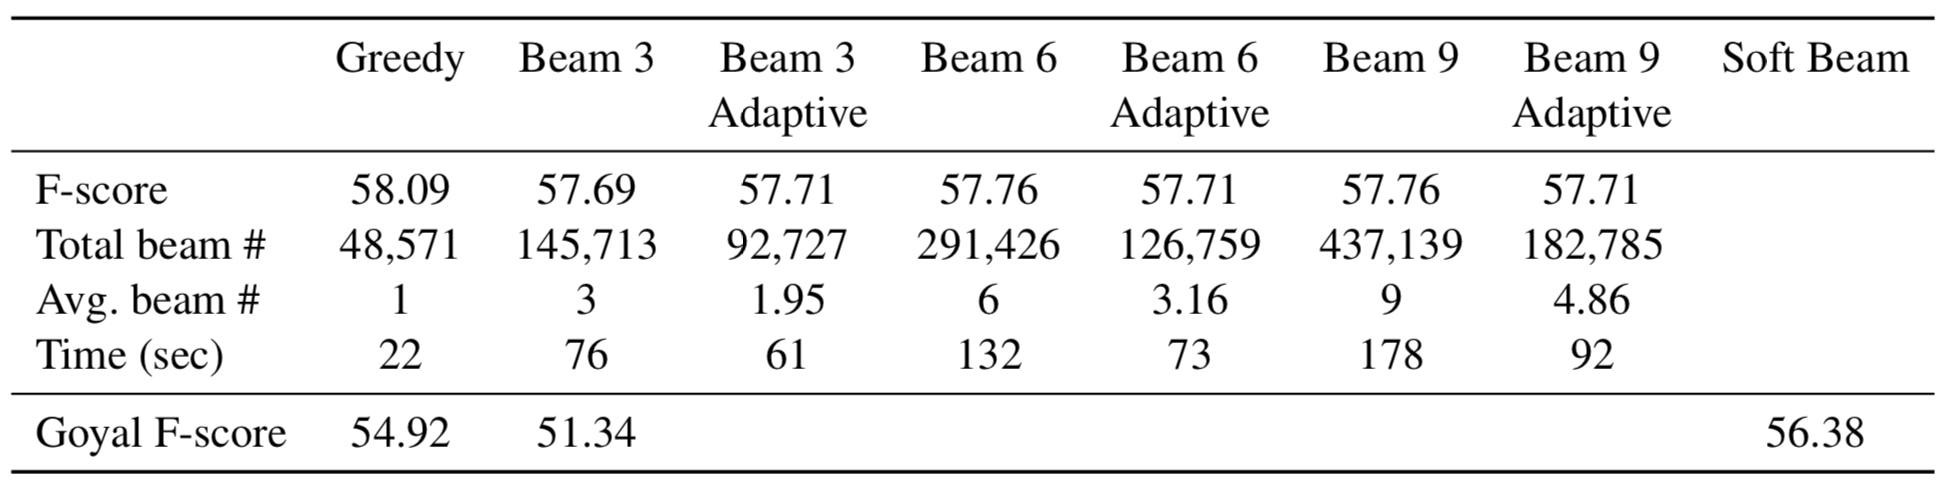
\includegraphics[width=0.9\linewidth]{det.png}
\end{center}

\begin{itemize}[leftmargin=*]
\item Results of Asynchronous Actor-Critic (adapt from given initial beam size):
\end{itemize}

\begin{center}
    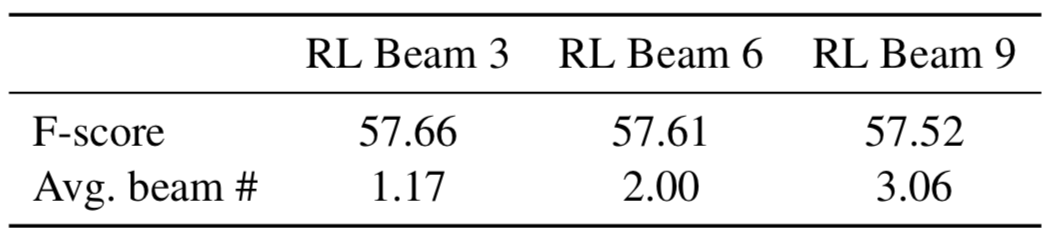
\includegraphics[width=0.5\linewidth]{rl.png}
\end{center}

}


\headerbox{8.~Future work}{name=conclusion,column=0,below=beam,span=1}{
% DeCAF is a chemoinformatical tool that can be helpful in ligand-based drug design.
% It provides a comprehensive molecule description and a fast algorithms for comparing and aligning multiple ligands.
\begin{itemize}[leftmargin=*]
\item Refine reinforcement learning techniques
\item Pre-train the Actor-Critic model with Deterministic Agent (using Imitation Learning)
\end{itemize}

%\begin{boenumerate}\compresslist
%    \item DeCAF gives better results for 23 out of 35 receptors.
%    \item For targets with easily separable active and inactive datasets, SEA and DeCAF give similar results.
%    \item In cases in which SEA fails to identify active molecules, our method performs substantially better.
%\end{boenumerate}
% It can be also used in other [procedures], such as database screening or drug repositioning.
% DeCAF is written in Python and freely available at \textbf{\color{darkgreen}http://bitbucket.org/marta-sd/decaf}. 
}


\headerbox{9.~References}{name=references,column=0,span=1,below=conclusion,above=bottom}{


%\small % Reduce the font size in this block
\renewcommand{\section}[2]{\vskip 0.05em} % Get rid of the default "References" section title
%\nocite{*} % Insert publications even if they are not cited in the poster


\bibliographystyle{unsrt}

% \small{
\bibliography{posterbib} % Use sample.bib as the bibliography file
% }

}

\end{poster}

\end{document}
